\section{Data} \label{sec:data}
The data used in this study were obtained using the Bench for Optical Testing (BOT), which was constructed and designed at SLAC National Accelerator Laboratory. The BOT enables laboratory tests with the LSSTCam, ensuring that flat images exhibit variations of less than 5\% for accurate measurements of linearity, FWC, and gain from the PTCs \citep{2018SPIE10702E..58N}. Figure \ref{fig:BOT_stand} illustrates the structure of the BOT, with the cryostat located at the circular top and the focal plane pointing downwards on the test bench.

\begin{figure}[!htb]
    \centering
    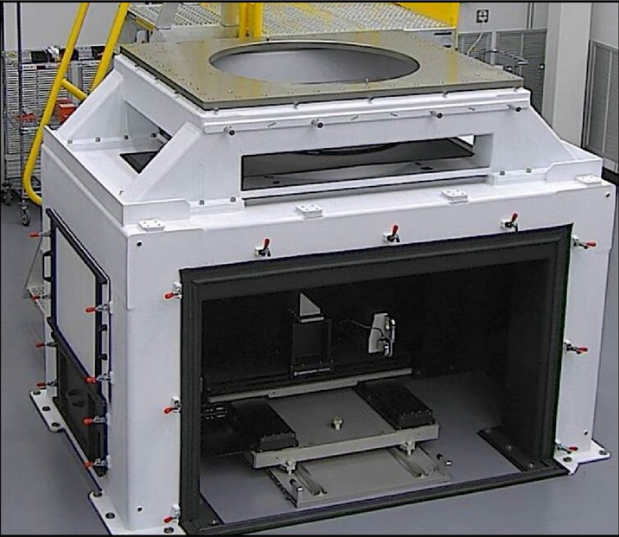
\includegraphics[width=0.7\textwidth]{Figures/BOT_stand.png}
    \caption{Bench for Optical Testing (BOT) designed by SLAC. Figure is taken from \cite{2018SPIE10702E..58N}. }
    \label{fig:BOT_stand}
\end{figure}

The data for this study were obtained from \textit{run 13144} and \textit{run 13186}, with the latter containing the crosstalk matrix information. As described in \cite{2020SPIE11454E..39S}, electronic crosstalk measurements were conducted using a projector known as the \textit{crosstalk projector}, which illuminates a single sensor with a collimated beam of light with a pattern containing large bright spots, each with a radius of 80 pixels. However, for laboratory tests simulating realistic source sizes, the \textit{spot grid projector}, an optical projector, was used. This projector generates spots in specific grids and includes filters to simulate both satellite trails and the signal level of the sky background.